\documentclass[article,english]{stucosrec}

% for testing purposes only
\usepackage{lipsum}

% Example of defining a new command
\newcommand{\latex}{\LaTeX\xspace}
\newcommand{\bibtex}{Bib\TeX\xspace}
\newcommand{\stucosrec}{StuCoSReC\xspace}
\newcommand{\latexe}{\LaTeX$2_\epsilon$\xspace}

\title{\latex TEMPLATE FOR \stucosrec CONTRIBUTION}
\author{
	Klemen Berkovi\v{c}\thanks{If this author has more email addresses you can add them here. Example email1@email.com, email2@email.si} \\
	Faculty of Electrical \\Engineering and Computer Science,\\
	University of Maribor,\\
	Koro\v{s}ka cesta 46, 2000 Maribor, Slovenia \\
	\texttt{klemen.berkovic1@um.si}
	\And
	Iztok Fister Jr.\thanks{If this author has more affiliation you can add them here. If there are multiple corresponding authors tell that in this section.} \\
	Faculty of Electrical \\Engineering and Computer Science,\\
	University of Maribor,\\
	Koro\v{s}ka cesta 46, 2000 Maribor, Slovenia \\
	\texttt{iztok.fister1@um.si}
	\AND
	Iztok Fister \thanks{If this author has telephone number you can add it here. In the telephone number include country code. Example +xx-xxxx-xxx-xxxx} \\
	Faculty of Electrical \\Engineering and Computer Science,\\
	University of Maribor,\\
	Koro\v{s}ka cesta 46, 2000 Maribor, Slovenia \\
	\texttt{iztok.fister@um.si}
}

% images directory
\imagespath{ {./images/} }

\begin{document}
	
	\maketitle
	
	\begin{abstract}
		This paper provides a sample of a \latex document which conforms to the formatting guidelines for \stucosrec Proceedings.
		It is a guide to Preparing \stucosrec Proceedings using \latexe and \bibtex.
		This source file has been written with the intention of being compiled under \latexe and \bibtex.
		The developers have tried to include every imaginable sort of ``bells and whistles", such as a subtitle, footnotes on title, subtitle and authors, as well as in the text, and every optional component (e.g. Review, Additional Authors, References, Acknowledgment) not to mention examples of equations, Tables, Figures, lists and algorithms.
		To make best use of this sample document, run it through \latex and \bibtex, and compare the output of this document to your produced output document.
	\end{abstract}

	\keywords{\stucosrec Proceedings \and \latex \and text tagging\footnote{List three to ten pertinent keywords specific to the article; yet reasonably common within the subject discipline.}}

	\section{Introduction}
	
	The \textit{proceedings} are the records of a conference.
	\stucosrec seeks to give these conference by-products a uniform, high-quality appearance.
	To do this, \stucosrec has some rigid requirements for the format of the proceedings documents: There is a specified format (balanced  double columns), a specified set of fonts (Arial or Helvetica and Times Roman) in certain specified sizes (for instance, 11 point for body copy), specified size of margins 1.76 cm top, 2.54 cm bottom and 1.6 cm left and right; specified column width 8.71 cm with vertical spacing between the columns equal to 0.35 cm.
	
	The good news is, with only a handful of manual settings, the \latex document class file handles all of this for you.
	In addition, the author has to use \textbf{article} option for the provided document class to create an article.
	If the author would want to produce an abstract he/she must use \textbf{abstract} instead of \textbf{article} option for the provided document class.
	Papers presenting student research are being reviewed.
	Papers must be in English, so in addition to \textbf{article} option, add \textbf{english} option to the document class.
	Papers must provide sufficient details to allow the Program Committee to assess their merits.
	For sending the document to a review procedure, the author must use the \textbf{review} option for the provided document class, and when the document passes the review procedure, then the author should remove the \textbf{review} option.
	Submissions are limited to at most \textbf{four pages} in a \texttt{pdf} format.
	
	The remainder of this document is concerned with showing, in the context of an ``actual'' document, the \latex commands specifically available for denoting the structure of a proceedings paper, rather than with giving rigorous descriptions or explanations of such commands.
	
	\section{The \textit{Body} of The Paper}
	
	Typically, the body of a paper is organized into a hierarchical structure, with numbered or unnumbered headings for sections, subsections, sub-subsections, and even smaller sections.
	The command \texttt{{\char'134}section} that precedes this paragraph is part of such a hierarchy\footnote{Command {\texttt{\char'134 And}} or/and {\texttt{\char'134 AND}}, you have already used for positioning the authors for your paper.}. \latex handles the numbering and placement of these headings for you, when you use the appropriate heading commands around the titles of the headings.
	If you want a sub-subsection or smaller part to be unnumbered in your output, simply append an asterisk to the command name.
	Examples of both numbered and unnumbered headings will appear throughout the balance of this sample document\footnote{This is the second footnote. It starts a series of three foot notes that add nothing informational, but just give an idea of how footnotes work and look. It is a wordy one, just so you see how a longish one plays out.}.
	
	Because the entire article is contained in the \textbf{document} environment, you can indicate the start of a new paragraph with a blank line in your input file; that is why this sentence forms a separate paragraph.
	
	\subsection{Type Changes and \textit{Special} Characters}
	
	We have already seen several typeface changes in this sample.
	You can indicate italicized words or phrases in your text with the command \texttt{{\char'134}textit}; emboldening with the command \texttt{{\char'134}textbf} and typewriter-style (for instance, for computer code) with \texttt{{\char'134}texttt}.
	But remember, you do not have to indicate typestyle changes when such changes are part of the \textit{structural} elements of your 	article; for instance, the heading of this subsection will be in a sans serif typeface, but that is handled by the document class file. Take care with the use of the curly braces in typeface changes; they mark the beginning and end of the text that is to be in the different typeface.
	
	You can use whatever symbols, accented characters, or non-English characters you need anywhere in your document\footnote{A third footnote, here. Let's make this a rather short one to see how it looks.}; you can find a complete list of what is available in the \textit{\latex
	User's Guide}~\cite{Lamport:LaTeX}.
	
	\subsection{Math Equations}
	
	You may want to display math equations in three distinct styles: Inline, numbered or non-numbered display.
	Each of the three are discussed in the next sections.
	
	\subsubsection{Inline (In-text) Equations}
	
	A formula that appears in the running text is called an inline or in-text formula.
	It is produced by the \textbf{math} environment, which can be invoked with the usual \texttt{{\char'134}begin {\char'134}end} constructs or with the short form \textbf{\$$\cdots$\$}.
	You can use any of the symbols and structures, from $\alpha$ to $\omega$, available in \latex~\cite{Lamport:LaTeX}; this section will simply show a few examples of in-text equations in context.
	Notice how this equation: 
	\begin{math}\lim_{n\rightarrow \infty}x=0\end{math}, 
	set here in in-line math style, looks slightly different when set in display style.
	(See next section).
	
	\subsubsection{Display Equations}
	
	A numbered display equation -- one set off by a vertical space from the text and centered horizontally -- is produced by the \textbf{equation} environment.
	An unnumbered display equation is produced by the \textbf{displaymath} environment.
	
	Again, in either environment, you can use any of the symbols and structures available in \latex; this section will just give a couple of examples of display equations in context.
	First, consider the equation, shown as an inline equation above:
	\begin{equation}\lim_{n\rightarrow \infty}x=0.\end{equation}
	Notice how it is formatted somewhat differently in the \textbf{displaymath} environment.
	Now, we'll enter an unnumbered equation:
	\begin{displaymath}\sum_{i=0}^{\infty} x + 1\end{displaymath}
	and follow it with another numbered equation:
	\begin{equation}\sum_{i=0}^{\infty}x_i=\int_{0}^{\pi+2} f\end{equation}
	just to demonstrate \latex's capable handling of numbering.
	
	Next you will see an example of an unnumbered equation not in the \textbf{displaymath} environment, but in short form defined with \textbf{\$\$$\cdots$\$\$}.
	When $a \ne 0$, there are two solutions to $ax^2 + bx + c = 0$ and they are $$x_{1, 2} = \frac{-b \pm \sqrt{b^2-4ac}}{2a}.$$
	
	Here is an example of referencing an equation. Equation~\ref{equ:yannibel} is showing how to write cases in \latex.
	
	\begin{equation}
		\begin{aligned} 
			\mathrm{nr}(G_i,r) & = \label{equ:yannibel}
			\begin{cases}
				1  & \text{$r$ is played by one member of $G_i$}\\
				-2 & \text{$r$ is not played in $G_i$} \\
				-p & \text{$r$ is played by $p$ members in $G_i$}\\
			\end{cases}
		\end{aligned}
	\end{equation}
	
	\subsubsection{Long equations}
	
	When an equation is too long for one column use the \textbf{aligned} environment within the \textbf{equation} environment.
	For aligning the equation within the \textbf{aligned} environment use symbol \textbf{\&} as seen in Equation~\ref{equ:ho}.
	
	\begin{equation}
		\begin{aligned}
			O_{\max}& = w_1 \sum_{a=1}^{m} \sum_{b=a+1}^{n} (-\lvert\text{CPT}_a 
			-\text{CPT}_b\rvert)\\ 
			&\quad + w_2 \sum_{j=1}^{m} (\text{DIF}_j) + w_3 \sum_{j=1}^{m} 
			(\text{INT}_j/\sum_{x=1}^{n} x_{ij})
		\end{aligned}
		\label{equ:ho}
	\end{equation}
	
	\subsection{Citations}
	
	Citations to articles \cite{lecun2015deep, braams:babel, herlihy:methodology}, conference proceedings \cite{vrbancic2019transfer, clark:pct} or books \cite{salas:calculus, Lamport:LaTeX, fister2019computational} listed
	in the Bibliography section of your article will occur throughout the text of your article.
	You should use \bibtex to produce this bibliography automatically; you simply need to insert one of several citation commands with a key of the item cited in the proper location in the \texttt{.tex} file \cite{Lamport:LaTeX}.
	The key is a short reference you invent to identify each work uniquely; in this sample document, the key is the first author's surname and a word from the title.
	This identifying key is included with each item in the \texttt{.bib} file for your article.
	
	The details of the construction of the \texttt{.bib} file are beyond the scope of this sample document, but more information can be found in the \textit{Author's Guide}, and exhaustive details in the \textit{\latex User's Guide}\cite{Lamport:LaTeX}.
	
	This article shows only the plainest form of the citation command, using \texttt{{\char'134}cite}.
	This is what is stipulated in the ACM citation style specifications.
	No other citation format is endorsed.
	
	\subsection{Tables}
	
	Because Tables cannot be split across pages, the best placement for them is typically at the top of the page nearest their initial cite.
	To ensure this proper ``floating'' placement of Tables, use the environment \textbf{table} to enclose the Table's contents and the Table caption.
	The contents of the Table itself must go in the \textbf{tabular} environment, to be aligned properly in rows and columns, with the desired horizontal and vertical rules.
	Again, detailed instructions on \textbf{tabular} material are found in the \textit{\latex User's Guide}.
	
	Immediately following this sentence is the point at which Table~\ref{tab:table1} is included in the input file; compare the placement of the Table here with the Table in the printed \texttt{pdf} output of this document.
	
	\begin{table}
		\centering
		\caption{Frequency of Special Characters.}
		\label{tab:table1}
		\begin{tabular}{|c|c|l|} \hline
			Non-English or Math&Frequency&Comments\\ \hline
			\O & 1 in 1,000& Swedish names\\ \hline
			$\pi$ & 1 in 5& In math\\ \hline
			\$ & 4 in 5 & In business\\ \hline
			$\Psi^2_1$ & 1 in 40,000& Unexplained \\ \hline
		\end{tabular}
	\end{table}

	To set a wider Table, which takes up the whole width of the page's live area, use the environment \textbf{table*} to enclose the Table's contents and the Table caption.
	As with a single-column Table, this wide Table will ``float" to a location deemed more desirable.
	Immediately following this sentence is the point at which Table~\ref{tab:table2} is included in the input file; again, it is instructive to compare the placement of the Table here with the Table in the printed \texttt{pdf} output of this document.
	
	\begin{table*}
		\centering
		\caption{Some Typical Commands.}
		\label{tab:table2}
		\begin{tabular}{|c|c|l|} \hline
			Command&A Number&Comments\\ \hline
			\texttt{{\char'134}imagespath} & 200 & For directory of included images \\ \hline
			\texttt{{\char'134}table} & 300 & For tables\\ \hline
			\texttt{{\char'134}table*} & 400& For wider tables\\ \hline
		\end{tabular}
	\end{table*}
	
	\subsection{Figures}
	
	Like Tables, Figures cannot be split across pages; the best placement for them is typically the top or the bottom of the page nearest their initial cite\footnote{A fourth, and last, footnote.}.
	To ensure this proper ``floating'' placement of Figures, use the environment \textbf{figure} to enclose the Figure and its caption.
	
	This sample document contains examples of \texttt{.pdf} files to be displayable with \latex.
	Usage of this type of Figure element is seen in Figure~\ref{fig:circles}.
	
	\begin{figure}
		\centering
		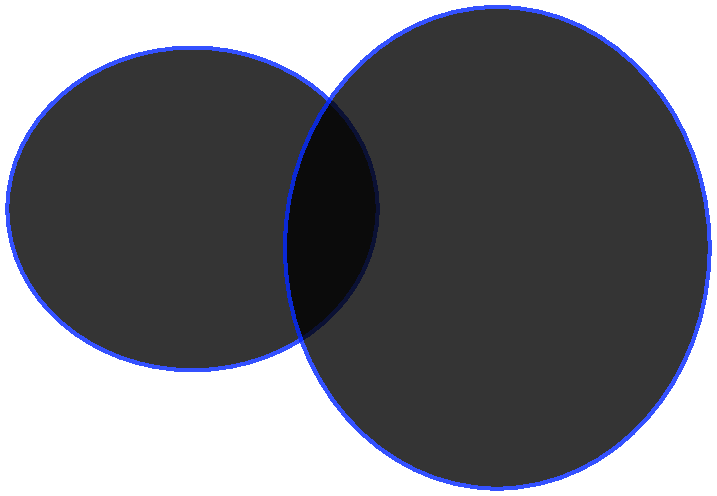
\includegraphics[scale=0.5]{circles.pdf}
		\caption{A sample circles graphic (\texttt{.pdf} format).}
		\label{fig:circles}
	\end{figure}

	This sample document contains examples of \texttt{.png} files to be displayable with \latex.
	Usage of this type of Figure element is seen in Figure~\ref{fig:star}.
	
	\begin{figure}
		\centering
		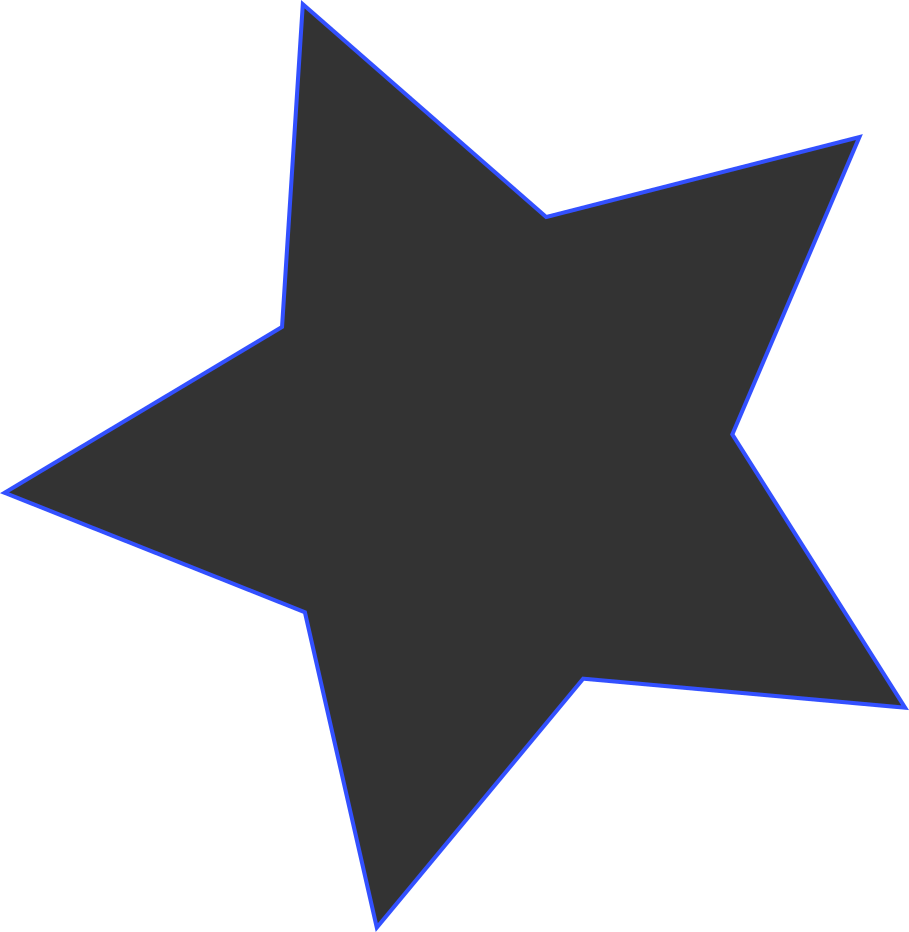
\includegraphics[scale=0.5]{star.png}
		\caption{A sample star graphic (\texttt{.png} format).}
		\label{fig:star}
	\end{figure}

	As was the case with Tables, you may want a Figure to span over two columns.
	To do this, and still to ensure proper ``floating'' placement of Tables, use the environment \textbf{figure*} to enclose the Figure and its caption.
	An example of this can be seen in Figure~\ref{fig:spin}.
	
	\begin{figure*}
		\centering
		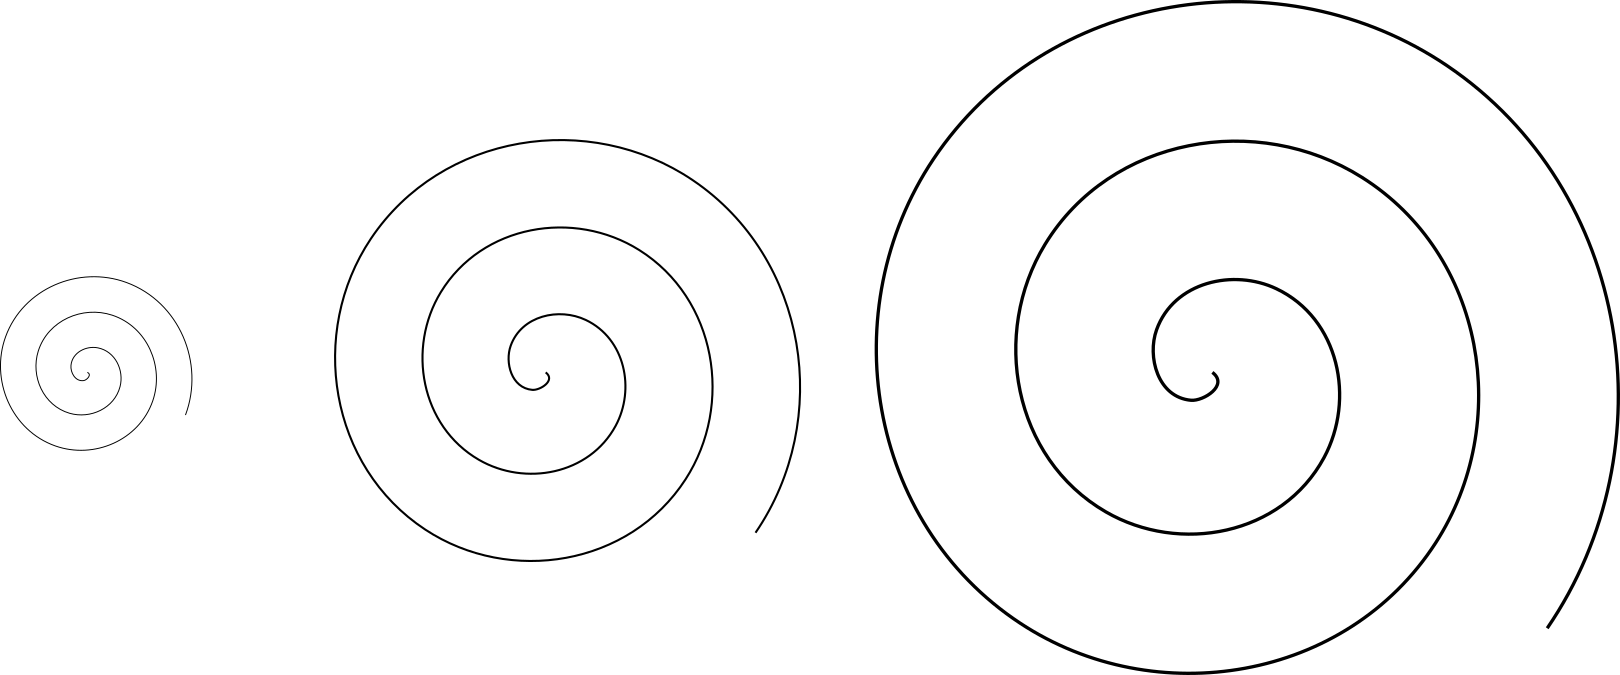
\includegraphics[scale=0.8]{spin.png}
		\caption{A sample spin graphic with a span.}
		\label{fig:spin}
	\end{figure*}
	
	\subsection{Lists}
	
	In the document you can use lists to present the information to the reader.
	Lists are created within the \textbf{itemize} \latex environment.
	In the next list example you can see how lists are created and used:
	
	\begin{itemize}
		\item First item,
		\item Second item and
		\item Third item.
	\end{itemize}
	
	Some times authors want to reference some list items in the later text.
	For that you can use \textbf{enumerate} \latex environment.
	An example of a numbered list:
	
	\begin{enumerate}
	    \item First point,
	    \item Second point,
	    \item $\cdots$
	\end{enumerate}
	
	And now reference Item 1, which is the first item in our list.

	\subsection{Algorithms}
	
	You may want to display algorithms in your document, check an example of an Algorithm~\ref{algo:sample}.
	Algorithms are written within the \textbf{algorithm} environment.
	
	\begin{algorithm}
		\SetAlgoLined
		\KwData{this text}
		\KwResult{how to write algorithm with \latexe}
		initialization\;
		\tcc{this is a comment to tell you that we will now really start code}
		\While{not at end of this document}{\label{algo:sample:while}
			read current\;
			\eIf{understand}{
				go to next section\;
				current section becomes this one\;
			}{
				go back to the beginning of current section\;
			}
		}
		\caption{How to write algorithms.}
		\label{algo:sample}
	\end{algorithm}

	You can reference a line in an algorithm which can be seen in the next sentence.
	An example of while loop can be seen in line~\ref{algo:sample:while}.
	For more details on the \textbf{algorithm} environment check \url{http://tug.ctan.org/macros/latex/contrib/algorithm2e/doc/algorithm2e.pdf} document.
	
	\section{Conclusions}
	
	This paragraph will end the body of this sample document.
	Remember that you might still have Acknowledgments; brief samples of these follow.
	There is still the Bibliography to deal with and we will make a disclaimer about that here: With the exception of the reference to the \latex book, the citations in this paper are to articles which have nothing to do with the present subject, and are used as examples only.
	
	\begin{acknowledgment}
		This section is optional; it is a location for you to acknowledge grants, funding, editing assistance and what have you.
		In the present case, for example, the authors would like to thank Klemen Berkovič for his help in codifying this \textit{Author's Guide}, the \texttt{.cls} and \texttt{.tex} files that is describes.
		The authors would like to thank Iztok Fister Jr. for his contribution to the \textit{Author's Guide} and \texttt{.tex} files.
	\end{acknowledgment}

	\bibliography{references}
	
\end{document}